\chapter{Development of the Prototype}\label{chapter:development_prototype}
\section{Requirements}\label{section:requirements}

In order to provide the blockchain-based weather insurance, our system must fulfill several key requirements. In this section we describe each category of requirements in a dedicated subsection.

\subsection{Functional Requirements}

\begin{itemize}
    \item \textbf{Policyholder Interaction}
    \begin{itemize}
        \item The system must provide a user interface for purchasing policies and control information such as whether a payment has been triggered or the payment status. 
        \item This user interface should be kept with minimum need
    \end{itemize}

    \item \textbf{Weather Data Integration} 
    \begin{itemize}
        \item The system must be able to receive and process global weather data from reliable and trusted external sources such as Global Surface Summary of the Day (GSOD) and Global Forecast System (GFS)
        \item Both historical and forecast data must be available
    \end{itemize}
    
    \item \textbf{Smart Contract}
    \begin{itemize}
        \item The smart contract must allow users to purchase weather-based insurance policies.
        \item The smart contract must store the policy terms, including the weather conditions that will trigger the specified amount of insurance payout.
        \item The contract must automatically trigger a payout when the predefined weather conditions are met.
    \end{itemize}
    
    \item \textbf{Oracle Integration}
    \begin{itemize}
        \item The system must use Chainlink oracles to retrieve and verify weather data from GCP datasets.
        \item Chainlink oracles must ensure secure transmission of data to the smart contract.
    \end{itemize}
    
    \item \textbf{Payout Processing}
    \begin{itemize}
        \item The system must be able to automatically execute payouts without manual intervention when the correct conditions are met.
    \end{itemize}
\end{itemize}

\subsection{Non-Functional Requirements}

\begin{enumerate}
    \item \textbf{Security}
    \begin{itemize}
        \item All the bilateral interactions between the smart contract, Chainlink oracle, google cloud and the user must be secure and tamper-proof.
    \end{itemize}
    
    \item \textbf{Scalability}
    \begin{itemize}
        \item The system must scale to handle multiple policies and users.
    \end{itemize}
    
    \item \textbf{Transparency}
    \begin{itemize}
        \item All transactions and insurance claims must be recorded on the blockchain for transparency and security.
    \end{itemize}
\end{enumerate}

\subsection{Technical Requirements (not finished)}

\begin{enumerate}
    \item \textbf{Blockchain Platform}
    \begin{itemize}
        \item The smart contract must be deployed on the Ethereum blockchain
    \end{itemize}
    
    \item \textbf{Data API}
    \begin{itemize}
        \item The system must use APIs to retrieve weather data from GCP.
    \end{itemize}
    
    \item \textbf{Chainlink Oracle}
    \begin{itemize}
        \item The system must integrate with a Chainlink node to facilitate data retrieval from GCP.
    \end{itemize}
\end{enumerate}

\section{Architecture}

In this section we will propose the architecture for our blockchain-based weather insurance system. First we present a high-level overview of the system and then elaborate on the most important components in a dedicated subsection for each component.

\subsection{General overview}

In \ref{fig:generalArchitecture} we present an overview of the general architecture that implements the requirements specified in \ref{section:requirements}. The center of the architecture is the smart contract deployed on the Ethereum blockchain. It manages all policies and decisions based on user requests and incoming weather data. The end user interacts directly with the smart contract through a decentralized app (see \ref{subsection:decentralizedApp}) where they can request insurance policies and track their contract status. 

The weather data is provided by Global Surface Summary of the Day (GSOD) and Global Forecast System (GFS) respectively. These datasets can be accessed via GCP BigQuery and GCP Storage through the GCP Interface. To bridge the gap between the off-chain data from GCP and the on-chain smart contract, the system uses a Chainlink Oracle (see \ref{subsection:ChainlinkOracle}). This Chainlink Oracle retrieves the weather data from GCP through the GCP Interface which are essentially API Endpoints and passes it on to the smart contract on the Ethereum blockchain.

\begin{figure}[h]
    \centering
    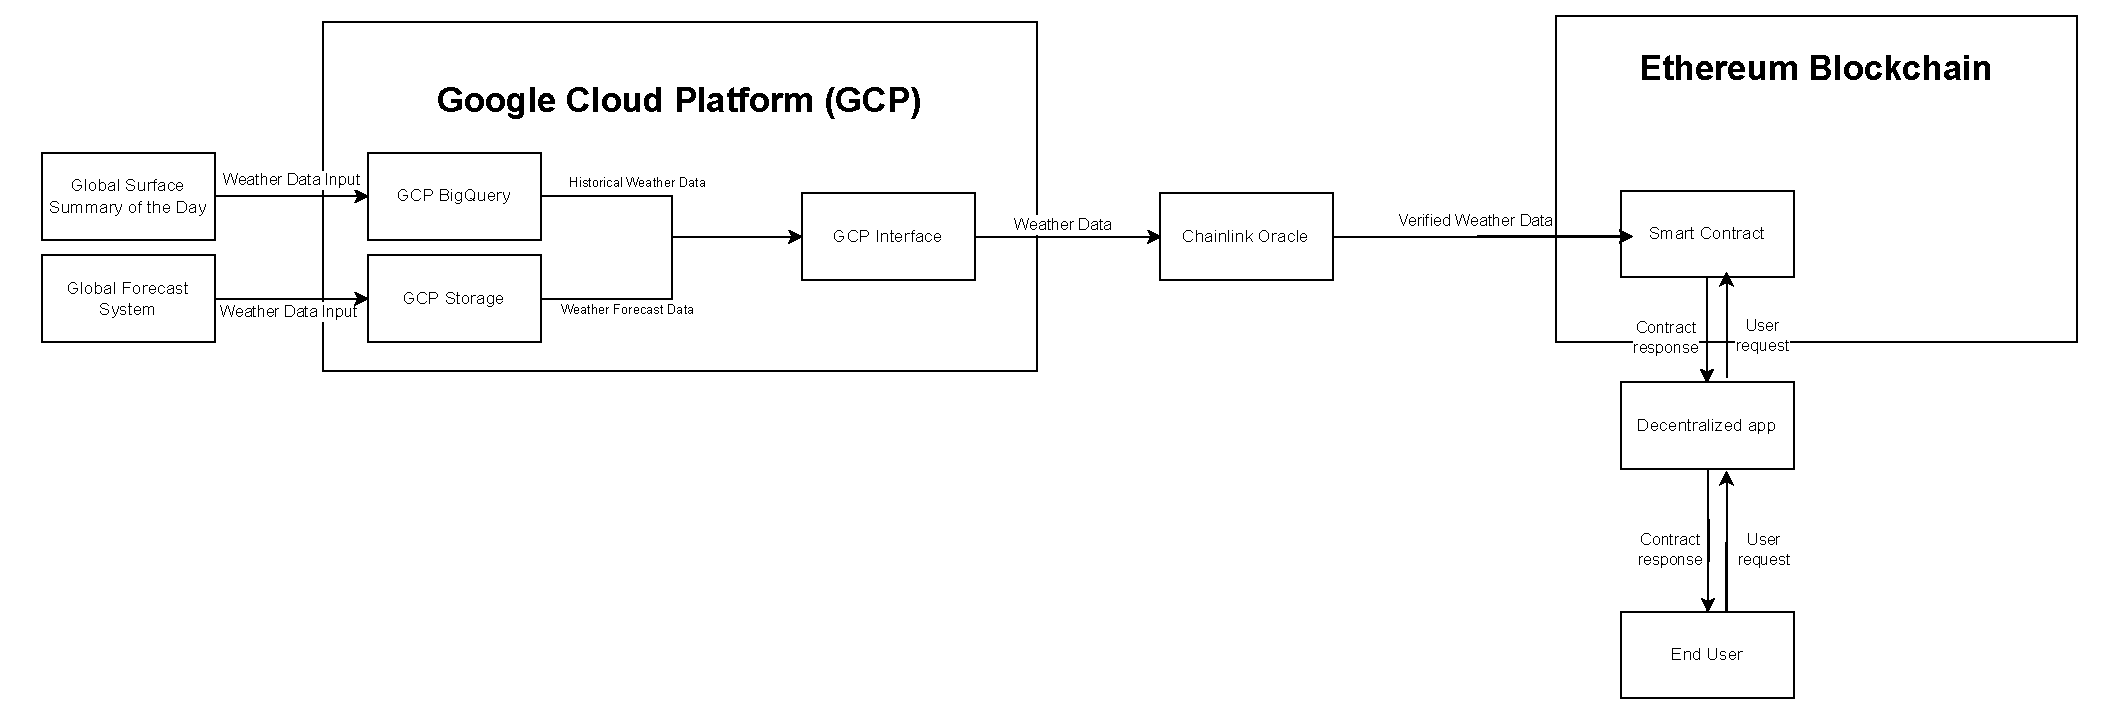
\includegraphics[width=0.8\textwidth]{figures/architecture-overview.drawio.pdf}
    \caption{Diagram showing the architecture of the smart contract. \textit{Source: Author's own representation.}}
    \label{fig:generalArchitecture}
\end{figure}

\subsection{Decentralized app}\label{subsection:decentralizedApp}

The decentralized application (DApp) allows a non-technical user to directly interact with the blockchain. Through its interface a user can request insurance policies, check policy statuses and receive notifications. Unlike traditional applications, which interact with a centrally managed backend, decentralized applications interact directly with a smart contract on a blockchain.

This interaction requires a digital wallet (e.g. MetaMask) which enables the user to initiate and sign a transaction when making a request, such as purchasing an insurance policy. In our architecture, the DApp serves as the primary interface in order for the end-users to interact with the system. 

(Idea: Include a mockup of a frontend utilizing metamask)

\subsection{Integration of chainlink oracles and GCP}\label{subsection:ChainlinkOracle}

Since the weater data from GSOD and GFS, which is accessed through the Google Cloud Platform (GCP), is not directly available from the on-chain environment of the smart contract we need to leverage oracles, which retreive and verify external data before delivering it to the blockchain.

In this case, Chainlink oracles are used to securely interact with the Google Cloud Platform (GCP) and pass it to the smart contract. The Chainlink oracle network consists of globally distributed nodes. When a request is triggered, multiple nodes independently access GCP and receive the weather data specified in the request. If any nodes return results that differ from the majority, they are flagged as potentially malicious. This decentralized approach ensures that only verified and reliable weather data is passed on to the smart contract.


\section{Data flow}

\subsection{General Flow}
\subsection{Interaction with smart contract}
\subsection{Smart contract fetching weather data}